\pagestyle{empty} % Limpa o cabeçalho e o rodapé
\onehalfspacing % Espaçamento entre-linhas de 1,5
% \hyphenpenalty=10000 % To prevent hyphenation
\pretolerance=10000 % To avoif overful lines
%\selectlanguage{english}
\selectlanguage{brazilian}
\setcounter{ex}{0} % counter for exercises
%\pagenumbering{arabic} % Uncomment this line if you want renumber pages for each chapter
\renewcommand{\chaptername}{Tutorial}
\chapter{Introdução à verossimilhança}\label{tut12}
\rhead{\tiny Instituto de Biociências --USP: BIZ0433 - Inferência Filogenética: Filosofia, Método e Aplicações}
\cfoot{\tiny \cc \ccby \ccsa \href{http://creativecommons.org/licenses/by-sa/4.0/}{Creative Commons Attribution-ShareAlike 4.0 International License}}
\vspace{5pt}
{\large \sc BIZ0433 - Inferência Filogenética: Filosofia, Método e Aplicações.}\par
{\sc Por \href{http://about.me/machadodj}{Denis Jacob Machado \& Fernando Marques}}\par
\vspace{10pt}
\par
\minitoc % for table of contents within the chapter
\newpage
\section*{}\addcontentsline{toc}{section}{Objetivo}
\onehalfspacing
\vspace*{5pt}
\begin{center}
\emph{\begin{large}Objetivo\end{large}}\label{tut12:Objetivo}
\vspace{2pt}
\end{center}

\begin{refsection}
\renewcommand*{\finalnamedelim}{\addspace\&\space} % Usar '&' ao invés de 'e'.

%% TEXTO DO RESUMO
Este tutorial introduz o conceito de verossimilhança como método de inferência e como ele pode ser aplicado como critério de otimalidade em inferência filogenética. Três tipos de verossimilhança são apresentados como critério de otimalidade. Finalmente, o conceito e a prática da seleção de modelos de substituição é apresentado. Os arquivos associados a este tutorial estão disponíveis em \url{http://lhe.ib.usp.br/cladistica}. Você pode baixá-los diretamente com o seguinte comando:

\begin{center}
\small \texttt{wget http://lhe.ib.usp.br/downloads/tutorial\_12.zip}\\
\end{center}


\newpage
\pagestyle{fancy} % Inclui o cabeçalho definido no meta.tex
%\pagenumbering{arabic} % Números das páginas em arábicos
%% color base pairs
\newcommand{\A}{\textcolor{green}{\textbf{A}}}
\newcommand{\C}{\textcolor{blue}{\textbf{C}}}
\newcommand{\G}{\textcolor{gray}{\textbf{G}}}
\newcommand{\T}{\textcolor{red}{\textbf{T}}}
\newcommand{\gap}{\textcolor{black}{\textbf{-}}}


%%%%%%%%%%%%%%%%%%%%%%%%%%%% HERE TEXT STARTS %%%%%%%%%%%%%%%%%%%%%%%%%%%%
\section{Probabilidades}\label{tut12:probs}
Há várias definições de probabilidades e uma breve consulta a literatura especializada revelará que não há consenso absoluto sobre esse conceito \parencite[considere a leitura de][, anexo ao diretório do tutorial]{Thacker_2014}. Independentemente do conceito que você adotar sobre probabilidade, há uma série de axiomas em Teoria de Probabilidades que você deve conhecer -- ou relembrar para que nós possamos entender os conceitos de verossimilhança. Neste tutorial iremos adotar a definição ``frequencista'' de probabilidades. Dentro deste contexto, dado $n$ eventos dentre os quais um conjunto de resultados mutuamente exclusivos ($E_{i}$) é observado, à medida em que $n \rightarrow \infty$, dizemos que a probabilidade de $E_{i}$ (isto é, $P_{(E_{i})}$) pode ser expressa por $E_{i}/n$. Há alguns axiomas da teoria de probabilidades, ou consequência desses, que você deve ter em mente:

\begin{center}
\begin{equation}
P_{(E_{i})} \geq 0;
\end{equation}
\end{center}

\begin{center}
\begin{equation}
P_{(E_{i})} = 1 - P_{(\tilde{E_{i}})};
\end{equation}
\end{center}

no qual $P_{(\tilde{E_{i}})}$ é a probabilidade de $P_{(E_{i})}$ não ocorrer,

\begin{center}
\begin{equation}
P_{(E_{i} { }ou{ } E_{j})} = P_{(E_{i} \cup E_{j})} = P_{(E_{i})} + P_{(E_{j})};
\end{equation}
\end{center}

assumindo que $E_{i}$ e $E_{j}$ sejam eventos disjuntos exclusivos, e

\begin{center}
\begin{equation}\label{eq:mult}
P_{(E_{i} e E_{j})} = P_{(E_{i} \cap E_{j})} = P_{(E_{i}) * P(E_{j})};
\end{equation}
\end{center}

no qual $E_{i}$ e $E_{j}$ são eventos eventos complementares independentes.

Por fim, probabilidades condicionais são expressas da seguinte forma:

\begin{center}
\begin{equation}
P_{(E_{i} \mid E_{j})} = \frac{P_{(E_{i} \cap E_{j})}}{P_{(E_{i})}};
\end{equation}
\end{center}

Neste caso, $P_{(E_{i} \mid E_{j})}$ denota a $P_{(E_{i})}$ ocorrer dado que $P_{(E_{j})}$ já ocorreu.
\\

\section{Princípios de estimativas de verossimilhança máxima}\label{tut12:estimate_ml}

Considere que você pegou uma moeda e jogou cara ou coroa 20 vezes e obteve o seguinte resultado \parencite[o mesmo exemplo é dado utilizando dictribuição binomial no Apêndice A de][]{anderson_2008}:
\begin{center}
Ca Co Co Ca Ca Ca Co Ca Co Co Co Ca Ca Co Ca Co Co Ca Ca Ca
\end{center}
ou seja 11 caras e 9 coroas. 

Qual seria a probabilidade desta observação ($P_{(obs)}$)?

Ela seria definida da seguinte forma:
\small
\begin{center}
$P_{(obs)} = P_{(Ca)}*P_{(Co)}*P_{(Co)}*P_{(Ca)}*P_{(Ca)}*P_{(Ca)}*P_{(Co)}*P_{(Ca)}*P_{(Co)}*P_{(Co)}*P_{(Co)}*P_{(Ca)}*P_{(Ca)}*P_{(Co)}*P_{(Ca)}*P_{(Co)}*P_{(Co)}*P_{(Ca)}*P_{(Ca)}*P_{(Ca)}$
\end{center}
\normalsize

ou seja (veja equação \ref{eq:mult}),

\begin{equation} \label{eq:prob1}
P_{(obs)} = P_{(Ca)}^{11}*P_{(Co)}^9
\end{equation}

Segundo a fórmula acima, e assumindo que a moeda não apresenta nenhum vício, você teria:

\begin{center}
$P_{(obs)} = 0.5^{11}*0.5^9 = 0.00000105415$
\end{center}

No entanto você assumiu que $P_{(Ca)} = P_{(Co)} = 0.5$. Suponha que você desconheça o valor de $P_{(Ca)}$ ou $P_{(Co)}$. Seria possível estimar esses valores? Estimativas de  Verossimilhança Máxima podem ser aplicadas nesse contexto.

Verossimilhança Máxima ($L$) é definida como:

\begin{equation} \label{eq:ml}
L_{(\theta | obs)} \propto P_{(obs | \theta)}
\end{equation}

onde, a Verossimilhança Máxima ($L$) de um parâmetro $\theta$ dado a observação é proporcional a probabilidade da observação dado um determinado parâmetro. Portanto, Verossimilhança Máxima lhe possibilita estimar o valor de $\theta$ que maximize a probabiliade de você observar os dados que observou.


Para aplicar Verossimilhança Máxima em nosso exemplo com caras e coroas, devemos considerar que:

\begin{center}
$P_{(Ca)}+P_{(Co)} = 1$
\end{center}
portanto,

\begin{equation} \label{eq:prob2}
P_{(Co)} = 1-P_{(Ca)}.
\end{equation}


Se considerarmos que a equação \eqref{eq:prob2} e a equação \eqref{eq:prob1} teríamos:


\begin{equation} \label{eq:prob3}
P_{(obs)} = P_{(Ca)}^{11}*(1-P_{(Ca)})^9
\end{equation}


Considere agora que o parâmetro $\theta$ que você gostaria de estimar é o valor de $P_{(Ca)}$ que maximizasse $L$. O valor de $P_{(Ca)}$ que maximizaria a probabilidade de observar seus dados seria definico como: 

\begin{equation} \label{eq:ml2}
L_{(P_{(Ca)} | obs)} \propto P_{(obs | P_{(Ca)})}
\end{equation}

Se você tem familiaridade com $R$, você pode usar o \textit{script} abaixo, disponível no diretório deste tutorial\footnote{ Você pode executar o seguinte comando ``\texttt{Rscript likelihood\_coin.r}'' e o script irá gerar o arquivo ``\texttt{Rplots.pdf}'' no qual existe um gráfico exemplificando a estimativa de verossimilhança máxima.}, para gerar os gráficos apresentados a seguir manipulando os valores de \textit{head} e \textit{tail}, para caras e coroas, respectivamente.

\begin{lstlisting}[label=tut3:ls1]
head <- 11   # mude aqui o numero de caras
tail <- 9   # mude aqui o numero de coroas
p <- seq(0,1,by=0.001)
for (i in p){L <- c((p^head)*(1-p)^tail)}
maxL <- max(L)
indexL <- match(maxL,L)
best_p <- p[indexL]
plot(p, L, xlab="P(Ca)", ylab="L", col="blue", frame=F, pch=16,cex=0.5)
text(0.8, maxL, paste("L =", maxL, "\n P(Ca) =", best_p))
\end{lstlisting}

A Figura \ref{fig:plot1} refere-se à nossa observação inicial e exibe os valores de $L$ associados com as possíveis probabilidades de caras (\textit{i.e.}, $P_{(Ca)}$) -- que varia de 0 a 1 em intervalos de 0.001).


%%%%%%%%%%%%%%%%%%%%%%%%%%% FIGURA DO GEDIT %%%%%%%%%%%%%%%%%%%%%%%%%%%
%  \vspace{-1em}
  \begin{figure}[h!]
    %\ffigbox[\FBwidth]
      {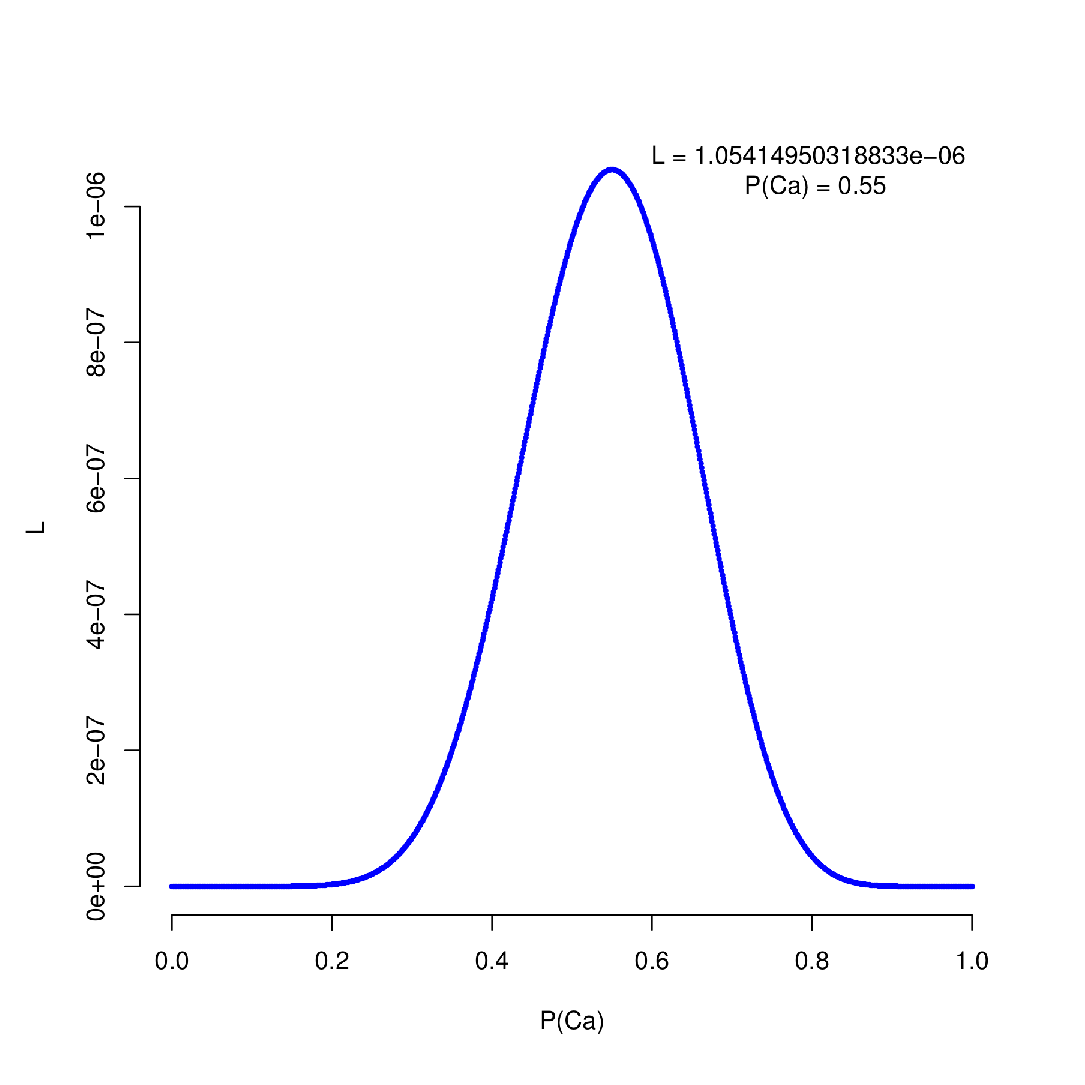
\includegraphics[scale=0.55]{figures/tut12/plot_1.eps}}
      {\caption{Valores de Verossimilhança ($L_{(P_{(Ca)}|obs)}$) em função da probabilidade de obter caras ($P_{(Ca)}$) para 20 eventos dos quais 11 resultaram em caras e 9 em coroas.}\label{fig:plot1}}
  \end{figure}

%%%%%%%%%%%%%%%%%%%%%%%%%%% FIM DA FIGURA DO GEDIT %%%%%%%%%%%%%%%%%%%%%%%%%%%

Observe que à medida em que $P_{(Ca)}$ se aproxima de 0.5, o valor de $L$ vai aumentando até chegar ao seu máximo. A Verossimilhança Máxima é obtida para $P_{(Ca)} = 0.55$. O que isso significa? De acordo com o conceito de Verossimilhança Máxima, a melhor estimativa de $P_{(Ca)}$ que explica sua observação (\textit{i.e.}, 11 caras e 9 coroas) é 0.55. Desta forma, o modelo probabilístico que melhor explica sua observação é $P_{(Ca)} = 0.55$ e $P_{(Co)} = 0.45$, o que significa que a moeda aparentemente não apresenta nenhum vício, pois essa diferença é muito pequena.\\

\stepcounter{ex}
\begin{blackBlock}{\textbf{Exercicio 13.\arabic{ex}}}\label{tut12:ex:13.1}

O que aconteceria se a observação fosse outra, como por exemplo, 3 caras e 17 coroas? A Figura \ref{fig:plot2} exibe os valores de $L$ associados com as possíveis probabilidades de caras para esta observação. Note como esse gráfico difere do primeiro. Você considera que o modelo que melhor explica essa observação sugere que a moeda é viciada? Justifique

\end{blackBlock}

\begin{center}
\line(1,0){400}\\
\line(1,0){400}\\
\end{center}

%%%%%%%%%%%%%%%%%%%%%%%%%%% FIGURA DO GEDIT %%%%%%%%%%%%%%%%%%%%%%%%%%%
%  \vspace{-1em}
  \begin{figure}[h!]
    %\ffigbox[\FBwidth]
      {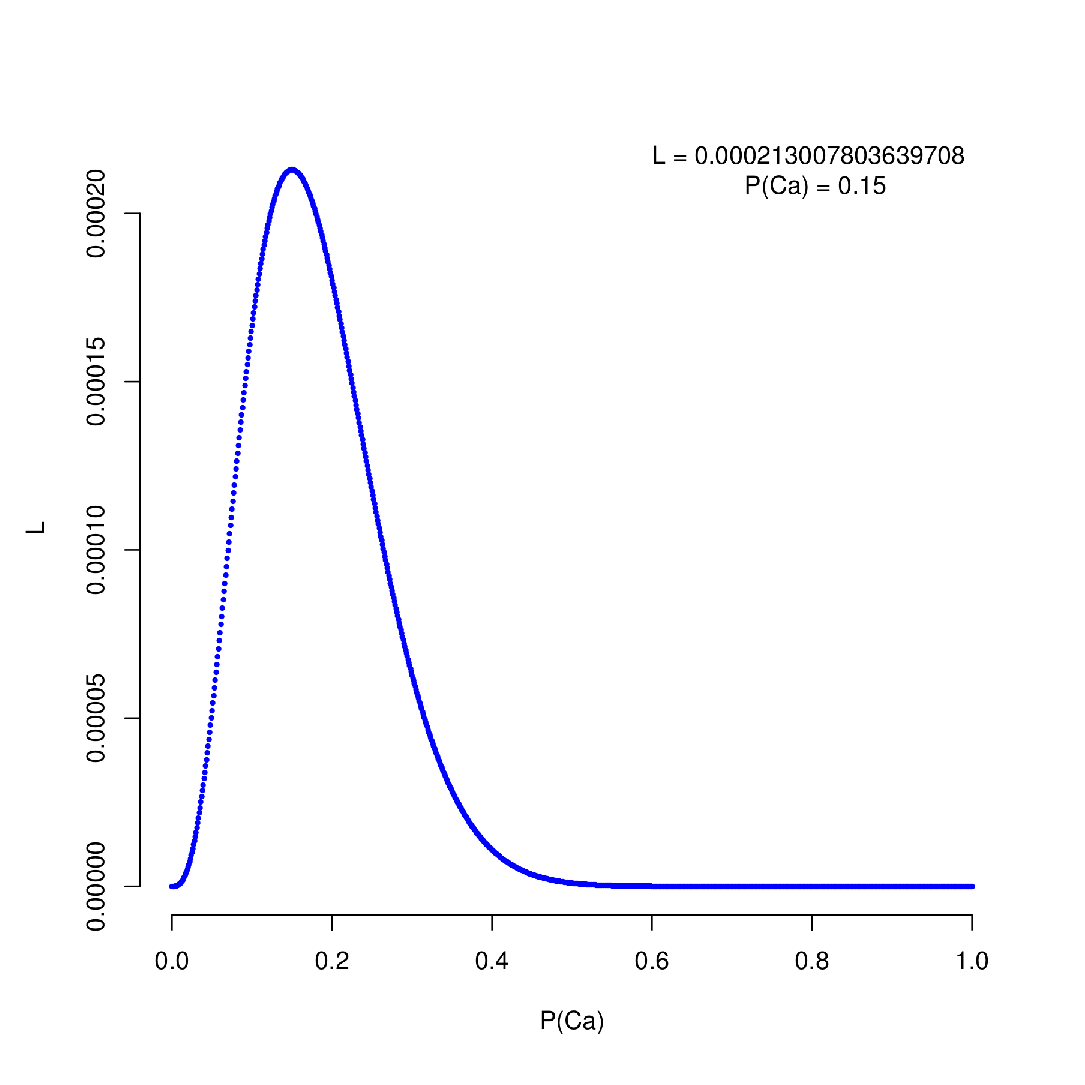
\includegraphics[scale=0.55]{figures/tut12/plot_2.eps}}
      {\caption{Valores de Verossimilhança ($L_{(P_{(Ca)}|obs)}$) em função da probabilidade de obter caras ($P_{(Ca)}$) para 20 eventos dos quais 3 resultaram em caras e 17 em coroas.}\label{fig:plot2}}
  \end{figure}

%%%%%%%%%%%%%%%%%%%%%%%%%%% FIM DA FIGURA DO GEDIT %%%%%%%%%%%%%%%%%%%%%%%%%%%

\stepcounter{ex}
\begin{blackBlock}{\textbf{Exercicio 13.\arabic{ex}}}\label{tut12:ex:13.2}

O gráfico abaixo representa os valores de Verossimilhança ($L$) dada a probabilidade de obter caras ($P_{(Ca)}$) em dois ensaios com 20 eventos de cara ou coroa. No primeiro ensaio, uma moeda resultou em 10 caras e 10 coroas (linhas pontilhadas). No segundo ensaio, uma outra moeda resultou em 3 caras e 17 coroas (linhas contínuas). Com base nestas informações, explique como Verossimilhança Máxima é usada para estimar parâmetros.

\end{blackBlock}

%%%%%%%%%%%%%%%%%%%%%%%%%%% FIGURA DO GEDIT %%%%%%%%%%%%%%%%%%%%%%%%%%%
%  \vspace{-1em}
  \begin{figure}[h!]
    %\ffigbox[\FBwidth]
      {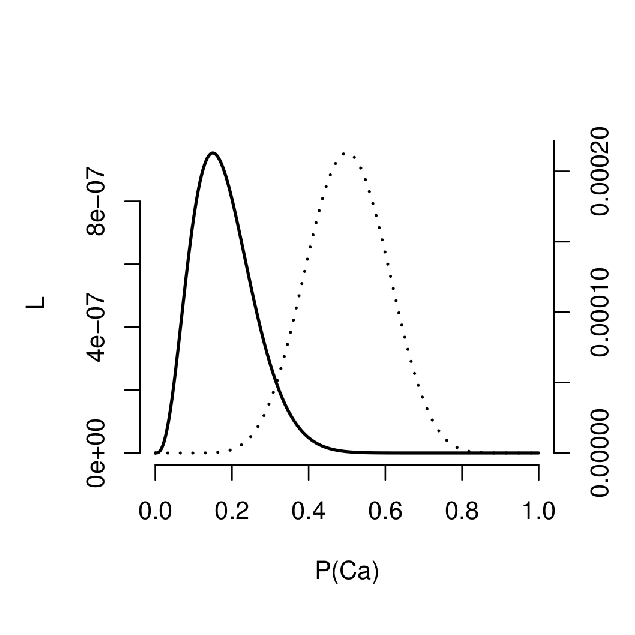
\includegraphics[scale=0.8]{figures/tut12/plot_coins.eps}}
      {\caption{Valores de Verossimilhança ($L_{(P_{(Ca)}|obs)}$) em função da probabilidade de obter caras ($P_{(Ca)}$).}\label{fig:plot_coin}}
  \end{figure}

%%%%%%%%%%%%%%%%%%%%%%%%%%% FIM DA FIGURA DO GEDIT %%%%%%%%%%%%%%%%%%%%%%%%%%%


\begin{center}
\line(1,0){400}\\
\line(1,0){400}\\
\line(1,0){400}\\
\end{center}



\section{Modelos de substituição}\label{tut12:mod}

A motivação pela qual \textcite{Felsenstein_1978} propôs o uso de estimativas de verossimilhança como critério de otimalidade em inferência filogenética veio da observação sob dados simulados de que topologias que possuíam comprimentos de ramos desproporcionais não eram recuperadas pelo critério da parcimônia. Desta forma, segundo o autor, a grande virtude do método proposto residia em considerar o comprimento de ramos durante a busca da melhor topologia.

Para considerar o comprimento de ramos é necessário a adoção de um modelo de substituição. De forma geral, o modelo estatístico é a formalização matemática da relação entre variáveis que correspondem a observações potenciais que inclui a descrição das incertezas sobre estas observações devido à variabilidade natural, erros ou informação incompleta. Neste caso em particular, esses modelos descrevem as probabilidades de transformação de caracteres dado sua frequência ($\pi$) e o comprimento de ramo ($v$). O comprimento deste ramo representa o número esperado de substituições por sítio e é definido por $v=3\alpha * t$; no qual $3\alpha$ é a taxa total de substituição e $t$ uma unidade de tempo qualquer. Uma vez que taxa e unidade de tempo estão interligados, arbitrariamente convencionou-se que a taxa receberia o valor de \textbf{uma substituição} que temos a expectativa que ocorra em \textbf{uma unidade de tempo} para cada sítio. Ao fazermos isso, ``tempo'' (o comprimento de um ramo) é medido em unidades de distância evolutiva (ou ainda, número de substituições esperada por sítio). Essa equivalência é feita assumindo que $\alpha = \frac{1}{3}$, pois teríamos $v = 3(\frac{1}{3})t$, ou seja, $v = t$.

Um dos modelos mais simples de substituição é conhecido como JC69 \parencite[][]{Jukes_and_Cantor_1969}. Este modelo assume que todas as bases são igualmente frequentes (0.25) e que a taxa de substituição ($\alpha$) é idêntica para todas as possíveis substituições cujos eventos obedecem a distribuição de probabilidades de Poisson. Esta distribuição descreve o número de ocorrências de um determinado evento aleatório (estocástico) em um determinado espaço de tempo, assumindo uma taxa média de ocorrência ($\lambda$).\footnote{Esta distribuição é derivada da distribuição binomial (veja \url{https://www.khanacademy.org/math/probability/random-variables-topic/poisson-process/v/poisson-process-1}).} 


 Desta forma, de acordo com esse modelo,

\begin{center}
\begin{equation}
P_{ij}(t) = \frac{1}{4}(1-e^{-4v/3}) = \frac{1}{4}-\frac{1}{4}e^{-4v/3}
\end{equation}
\end{center}

e

\begin{center}
\begin{equation}
P_{ii}(t) =  e^{-4v/3}+\frac{1}{4}(1-e^{-4v/3}) = \frac{1}{4}+\frac{3}{4}e^{-4v/3}
\end{equation}
\end{center}


onde $P_{ii}(t)$ é a probabilidade de não-mudança do estado de caráter durante o tempo $t$.


Considere por exemplo, a transformação da sequência ancestral \texttt{ACGTACGTACGT} para a sequência descendente \texttt{ACGTACGTAAAA} dado que $v$ é igual a 0.1. A probabilidade $P_{(ACGTACGTACGT \rightarrow ACGTACGTAAAA|\theta = v = 0.1)}$ seria:

\begin{center}
\begin{equation}
P_{(ACGTACGTACGT \rightarrow ACGTACGTAAAA|v = 0.1)} =  \bigg[\Big(\frac{1}{4}-\frac{1}{4}e^{-4(0.1/3)}\Big)^3\bigg]*\bigg[\Big(\frac{1}{4}+\frac{3}{4}e^{-4(0.1/3)}\Big)^9\bigg]
\end{equation}
\end{center}

ou seja,


\begin{center}
\begin{equation}
P_{(ACGTACGTACGT \rightarrow ACGTACGTAAAA|v = 0.1)} =  0.00001254686
\end{equation}
\end{center}

No entanto, talvez $v=0.1$ não seja o melhor valor deste parâmetro para explicar a transformação entre estas duas sequências. Usando o conceito de máxima verossimilhança poderíamos estimar o valore de $v$ que maximizaria $P_{(ACGTACGTACGT \rightarrow ACGTACGTAAAA|\theta = v)}$. O script \texttt{likelihood\_v.r}, disponível no diretório deste tutorial, computa os valores de $L_{(v|ACGTACGTACGT \rightarrow ACGTACGTAAAA)}$ -- como ilustrado na Figura \ref{fig:plot3}.

%%%%%%%%%%%%%%%%%%%%%%%%%%% FIGURA DO GEDIT %%%%%%%%%%%%%%%%%%%%%%%%%%%
%  \vspace{-1em}
  \begin{figure}[h!]
    %\ffigbox[\FBwidth]
      {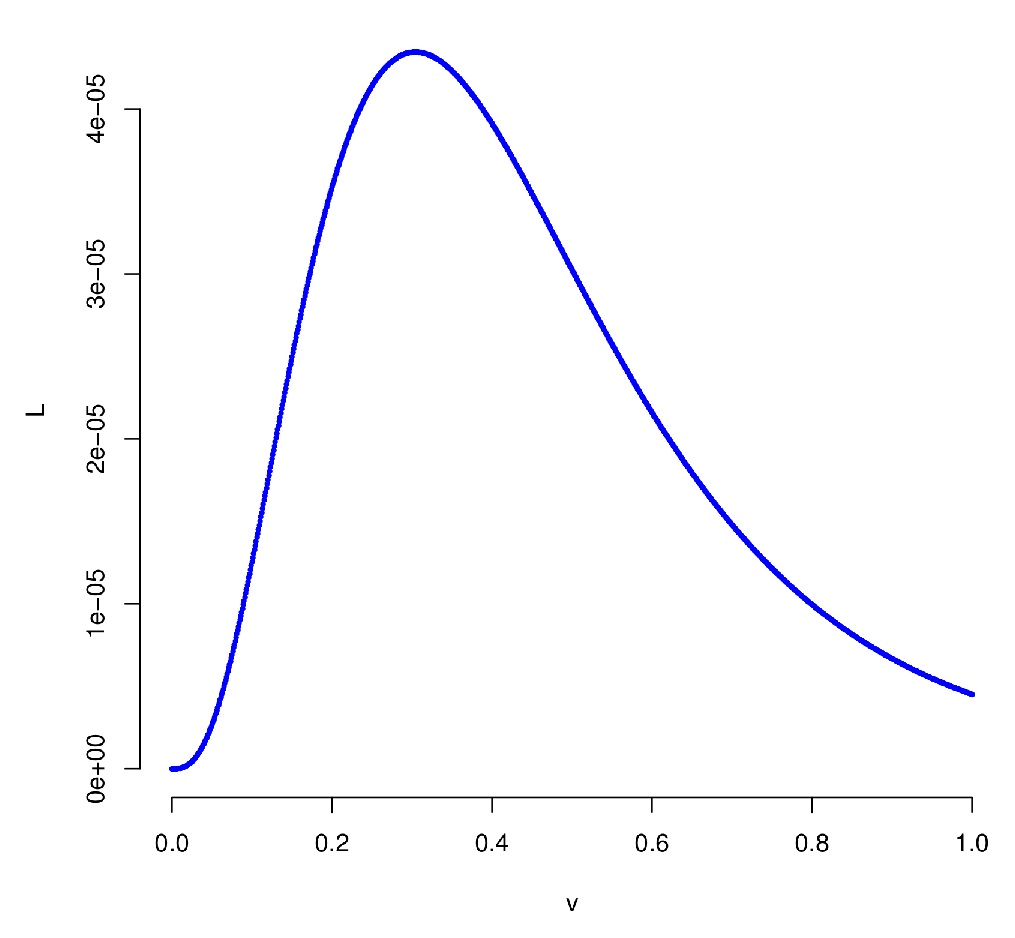
\includegraphics[scale=0.55]{figures/tut12/plot_3.eps}}
      {\caption{Valores de Verossimilhança ($L_{(v|obs)}$) em função do comprimento de ramo $v$.}\label{fig:plot3}}
  \end{figure}

%%%%%%%%%%%%%%%%%%%%%%%%%%% FIM DA FIGURA DO GEDIT %%%%%%%%%%%%%%%%%%%%%%%%%%%

\stepcounter{ex}
\begin{blackBlock}{\textbf{Exercicio 13.\arabic{ex}}}\label{tut12:ex:13.3}

Você considera que valor de $v$ utilizado anteriormente é uma boa estimativa para esse parâmetro? Justifique

\end{blackBlock}

\begin{center}
\line(1,0){400}\\
\line(1,0){400}\\
\end{center}


\section{Verossimilhança como critério de otimalidade} \label{tut12:first_sec}

Assim como em parcimônia (MP), a busca de árvores sob o critério de máxima verossimilhança (``maximum likelihood'', ML) assinala estados ancestrais (dentro de um contexto absoluto ou de médias) tal que a verossimilhança da árvore (hipótese) é maximizada. Para o conjunto de dados $D$, o modelo de substituição $\Theta$ e a topologia $T$:

\begin{center}
\begin{equation}
L_{(T, \Theta \mid D)} \propto P_{(D \mid T,\Theta)}
\end{equation}
\end{center}

Nesta expressão, uma determinada $T$ é selecionada de modo que $P_{(D \mid T,M )}$ é maximizada.

% Denis version
%O critério de máxima verossimilhança requer modelos específicos de evolução de caracteres (diferentemente dos regimes de custo que podem ser aplicados em parcimônia) e de parâmetros de ramos (comprimento de ramos; em parcimônica tais parâmetros não são requeridos), além de uma série de outros parâmetros conhecidos coletivamente como parâmetros inconvenientes (do inglês, ``nuisance parameters'').

\subsection{Parâmetros inconvenientes e medidas de máxima verossimilhança}

Os parâmetros inconvenientes são todos os demais parâmetros, fora $T$ e $D$, necessários para calcular $P_{(D \mid T)}$. Os três parâmetros inconvenientes mais importantes são: (\textit{i}) os parâmetros libres do modelo de substituição, (\textit{ii}) tempo e taxa de transformação nos ramos e (\textit{iii}) distribuição das taxas entre os caracteres. Estes parâmetros são coletivamente chamados $\theta$. Assumindo uma distribuição para os parâmetros inconvenientes $\Phi(\theta \mid T)$, pode-se integrar $\theta$ (dentro do espaço de parâmetros $\Theta$) para determinar $P_{(D \mid T)}$:

\begin{center}
\begin{equation}
P_{(D \mid T)} = \int_{(\theta \in \Theta)} P_{(D \mid T,\theta) d\Phi(\theta \mid T)}
\end{equation}
\end{center}

O $T$ que maximize $P_{(D \mid T)}$ desta maneira é chamado máxima verossimilhança integrada (``maximum integrated likelihood'', MIL) \parencite{Steel2000}. A MIL é igual à máxima probabilidade posterior (do inglês, ``maximum a posteriori'', MAP) quando a distribuição assumidas a priori (``\textit{priors}'') for uniforme (``flat'').

Como $\theta$ é composto de muitos parâmetros de distribuição desconhecida, uma abordagem para lidar com estes parâmetros é selecionar $\theta$ tal que $P_{(D \mid T,\theta)}$ seja maximizada. Isto equivale à máxima verossimilhança relativa (do inglês ``maximum relative likelihood'', MRL). A MRL é a metodologia mais usada em análises empíricas. Seu cálculo independe de $P_{(T)}$ e $\Phi_{(\theta \mid T)}$. Os tipos de MRL estão listados abaixo:

\begin{itemize}
\item ``Maximum average likelihood''~\parencite[MAL, ][]{Barry&Hartigan1987}: soma sobre todos os possíveis estados dos vértices. Esta forma de verossimilhança é a mais comumente empregada em análises empíricas.
\item ``Most parsimonious likelihood''~(MPL, também conhecida como ``ancestral maximum likelihood''): valores e parâmetros específicos são atribuídos para cada vértice. Apesar de se parecer em alguns aspectos com uma análise de parcimônia, MPL e parcimônia não convergem pois todas as taxas aplicadas sobre os ramos serão as mesmas para todos os caracteres.
\item ``Evolutionary path likelihood''~\parencite[EPL, ][]{Farris1973EPL}: toda sequência de estados de caracter intermediários entre os vértices é especificada de tal modo que a verossimilhança de toda árvore é maximizada. A árvore que maximiza EPM é a árvore mais parcimoniosa.
\end{itemize}

%\begin{blackBlock}{\textbf{Pergunta 1}}
%a) MP é uma forma de ML?
%
%b) Os modelos em ML são equivalentes aos regimes de custo em MP?
%\end{blackBlock}

%\begin{center}
%\line(1,0){400}\\
%\line(1,0){400}\\
%\line(1,0){400}\\
%\line(1,0){400}\\
%\line(1,0){400}\\
%\end{center}

\subsection{Calculando $P_{(D \mid T,\theta)}$}

Para um único caráter ($x$) em uma árvore, a verossimilhança do vértice $i$ ($Li$) com vértices descendentes $j$ e $k$ será a soma da probabilidade entre $xi$ e cada um de seus descendentes (dado um comprimento de ramo $v$) multiplicadas por suas respectivas verossimilhanças e somadas para todos os estados. A verossimilhança dos caracteres é multiplicada sobre todo o conjunto de dados para determinar a verossimilhança.

\begin{center}
\begin{equation}
L_{i}(x) = \sum_{i}^{estados} \left[\left(\sum_{x_j}p_{x_i,x_j}(v_j)L_j(x_j)\right) \times \left(\sum_{x_k}p_{x_i,x_k}(L_k)(x_k)\right)\right]
\end{equation}
\end{center}

Usando dados reais, os comprimentos dos ramos são quase sempre desconhecidos e precisam ser estimados. Isto pode ser feito de diversas maneiras mas normalmente depende da probabilidade marginal (mantendo todos os demais parâmetros constantes) de um dado ramo assumindo uma variedade de valores (parâmetro $v$) e escolhendo um valor ótimo \parencite[para mais detalhes, veja ][, Capítulo 11]{Wheeler2012}.

O cálculo da MAL de uma árvore é um procedimento heurístico devido ao grande número de parâmetros que devem ser estimados. Assim como em parcimônia, a árvore é obtida assinalando estados medianos recursivamente. Este procedimento é inicializado assinalando um valor igual a 1 para todos os ramos terminais. A verossimilhança é determinada dos ramos terminais para a raiz, multiplicando-se pelas probabilidades \textit{a priori} dos próprios estados.

\begin{center}
\begin{equation}
L_{T}(x) = \prod_{i=1}^{estados} \pi_{i} \prod_{\forall u,v \in E} L_{u,v}
\end{equation}
\end{center}

Dado que estes valores são geralmente muito baixos, é geralmente mais conveniente expressá-los em forma logarítmica.

\subsection{Exemplo simples}

Considere um único nucleotídeo caracterizado sob o model JC69. As probabilidades de ramo serão ficadas em $v = \mu t=0.1$.

\begin{center}
\begin{equation}
f(n) = \left\{
  \begin{array}{l l}
    \dfrac{1}{4} + \dfrac{3}{4}e^{-\mu t} & \quad \text{i $=$ j}\\
    \dfrac{1}{4} - \dfrac{1}{4}e^{-\mu t} & \quad \text{i $\neq$ j}
  \end{array} \right.
\end{equation}
\end{center}

Deste modo, as probabilidades de ramo são:

\begin{center}
\begin{equation}
f(n) = \left\{
  \begin{array}{l l}
    0.929 & \quad \text{i $=$ j}\\
    0.0238 & \quad \text{i $\neq$ j}
  \end{array} \right.
\end{equation}
\end{center}

Veja na \textbf{Figura~\ref{tut12:fig:exemplo}} como seria o cálculo da sub-árvore à seguir com ramos terminais contendo os caracteres A e C e parâmetro de ramo $0.1$. A verossimilhança média da árvore é $1,76 \times 10^{6}$ ou, em $-log$ (base $e$), $13,25$.

%  \vspace{-1em}
  \begin{figure}[H]
    %\ffigbox[\FBwidth]
      {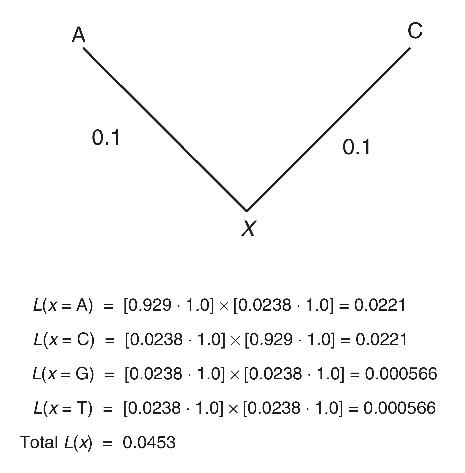
\includegraphics[scale=1.0]{figures/tut12/exemplo.eps}}
	{\caption[Sub-árvore anotada com cálculo de verossimilhança]{Sub-árvore anotada com cálculo de verossimilhança (de Wheeler, 2012: Fig. 11.8).}\label{tut12:fig:exemplo}}
  \end{figure}


\stepcounter{ex}
\begin{blackBlock}{\textbf{Exercicio 13.\arabic{ex}}}\label{tut12:ex:13.4}

Qual seria a verossimilhança da sub-árvore da figura acima caso ``gaps''(inserções/ deleções, ou ``InDels'') fossem tratados como um quinto estado de caráter e o parâmetro dos ramos fosse 0.2?

\end{blackBlock}

\begin{center}
\line(1,0){400}\\
\line(1,0){400}\\
\line(1,0){400}\\
\line(1,0){400}\\
\line(1,0){400}\\
\end{center}

\subsection{Seleção de modelos e dados lacunares}\label{tut12:first_sec:model}

A adoção do critério de verossimilhança em inferência filogenética requer a escolha de um modelo probabilístico de substituição. Quanto maior é o número de parâmetros livres em um modelo -- aqueles são estimados durante a análise--, maior será o ajuste do modelo aos seus dados, no entanto você pode usar parâmetros desnecessários, cuja a inclusão não justifica o ganho no valor de verossimilhança. Desta forma, o procedimento de seleção de modelos, visa adotar o modelo com o menor número de parâmetros livres que de acordo com critérios que visam penalizar a sobre-parametrização de modelos.

A escolha destes modelos deve preceder a análise filogenética e deve ser feita de forma objetiva \parencite[veja conceitos e referências em][]{Darriba_and_Posada_2015}. Neste tutorial nos iremos adotar como critério de escolha de modelos o critério de informação de Akaike corrigido (\textit{Akaike Information Criteria -- $AIC_{c}$}). Esta métrica não corrigida é computada da seguinte forma:

\begin{center}
\begin{equation}\label{tut12:first_sec:model_aic}
AIC = -2l + 2k
\end{equation}
\end{center}

no qual $l$ é o log da verossimilhança e $k$ é o número de parâmetros livres do modelo -- aqueles que são maximizados na função de verossimilhança. Vale ressaltar que o $k$ inclui os parâmetros livres do modelo de substituição \parencite[veja Tabela 1 de][]{Darriba_and_Posada_2015}, mais a topologia e seus comprimentos de ramos (\textit{i.e.}, $(t * 2)-3$, onde $t$ é o número de terminais). Sua correção é necessária quando o número amostral -- neste caso número de caracteres $n$ -- é pequeno quando comparado com o número de parâmetros livres (\textit{i.e.}, estimados; digamos $\frac{n}{k} < 40$) e é dada pela fórmula:

\begin{center}
\begin{equation}\label{tut12:first_sec:model_aicc}
AIC_{c} = AIC + \frac{(2k(k-1))}{(n-k-1)}
\end{equation}
\end{center}

Em principio, dados lacunares (``missing data'') não são um problema para análises de verossimilhança. Estados de ramos terminais podem ser definidos com probabilidade de transformação igual a 1.0 para cada estado observado ou implícito. Porém, diferentes implementações podem diferir na forma de tratar estes dados. É evidente que a implementação de dados lacunares irá afetar as análises. Este problema torna-se ainda mais pernóstico quando INDELS (\textit{i.e.}, inserções e deleções) são tratados como dados lacunares. Este tratamento é problemático, porém matematicamente necessário para manter o cálculo da verossimilhança factível dentro dos limites atuais de tempo e recursos computacionais.

Nos exercícios abaixo você deverá selecionar modelos para dois bancos de dados, incluindo três alinhamentos distintos. O objetivo é verificar como alinhamentos modificam os critérios de escolha de modelos e refletir sobre o uso de $AIC_{c}$ em análises por verossimilhança máxima.\\


\stepcounter{ex}
\begin{blackBlock}{\textbf{Exercicio 13.\arabic{ex}}}\label{tut12:ex:13.5}

Neste exercício você deverá fazer três linhamentos distintos para as sequências no arquivo \texttt{partition2.fas} (\textit{i.e.}, \texttt{partition2aln1.fas}, \texttt{partition2aln2.fas} e \texttt{partition2aln3.fas}) utilizando \texttt{MAFFT} e os seguintes parâmetros de alinhamento: abertura de gaps (\texttt{{-}{-}op})  $3.06$, $1.53$ e $0.123$ no qual o valor dos gaps de extenção (\texttt{{-}{-}ep})  será fixado em $0.123$ (veja Seção \ref{tut8:msa:mafft} do Tutorial \ref{tut8} caso tenha dúvidas).

\end{blackBlock}

\begin {myindentpar}{0.3cm}
\begin{enumerate}[\itshape i.]
	\item{Qual valor de ``gap opening'' resultou em um alinhamento com mais gaps? Porquê?}

\begin{center}
\line(1,0){400}\\
\line(1,0){400}\\
\line(1,0){400}\\
\end{center}

\end{enumerate}
\end{myindentpar}

\begin{comment}
% isso era o texto da versão anterior a 2018 no qual usava-se jModelTest para seleção modelos

Vejamos como esses alinhamentos influenciam a seleção de modelos de substituição. Para a seleção de modelos utilizaremos o aplicativo \href{http://code.google.com/p/jmodeltest2/}{jModelTest 2} \parencite[][]{Darriba_et_al_2012,Guidon_and_Gascuel_2003}. Operacionalmente, o cálculo de $AIC_{c}$ para cada modelo em \href{http://code.google.com/p/jmodeltest2/}{jModelTest 2} é relativamente simples, no entanto recomendo a leitura do manual do programa \parencite[][]{Darriba_and_Posada_2015} e as referência citadas no mesmo caso tenha interesse em entender aspectos metodológicos e filosóficos mais detalhados associados ao método. Adicionalmente, para que obtenham uma visão mais ampla sobre complexidades de modelos e critérios de seleção, eu sugiro fortemente a leitura dos capítulos pertinentes de \textcite{anderson_2008}. Este livro, embora escrito fora do contexto de análises filogenéticas, lhes fornecerão uma visão global sobre o tema.\\
\end{comment}

Existem algumas ferramentas para a seleção de modelos em análises filogenéticas, sendo \href{http://code.google.com/p/jmodeltest2/}{jModelTest 2} \parencite[][]{Darriba_et_al_2012,Guidon_and_Gascuel_2003} uma das mais tradicionais e a leitura do manual deste programa pode ser muito instrutiva. No entanto, o programa \href{http://www.iqtree.org/}{IQ-TREE} \parencite{Nguyen_et_al_2015} -- um aplicativo relativamente recente -- tornou o jModelTest 2 obsoleto na minha opinião. O \href{http://www.iqtree.org/}{IQ-TREE} possibilita a avaliação de um maior número de modelos e é muito mais rápido e robusto que o jModelTest 2.

O \href{http://www.iqtree.org/}{IQ-TREE} utiliza o algoritmo do ModelFinder \parencite{kalyaanamoorthy_et_al_2017} para a seleção de modelos e maiores detalhes sobre a seleção de modelos em IQ-TREE podem ser encontrados nos tutoriais do programa -- na seção \href{http://www.iqtree.org/doc/Tutorial#choosing-the-right-substitution-model}{``Choosing the right substitution model''} e/ou na documentação do programa -- na seção \href{http://www.iqtree.org/doc/Substitution-Models}{``Substitution models''}.\\


\stepcounter{ex}
\begin{blackBlock}{\textbf{Exercicio 13.\arabic{ex}}}\label{tut12:ex:13.6}

Neste exercício você deverá computar os parâmetros de seleção de modelos para o arquivo \texttt{partition1.fas} -- que não requer alinhamento -- e os três linhamentos distintos para as sequências no arquivo \texttt{partition2.fas} (\textit{i.e.}, \texttt{partition2aln1.fas}, \texttt{partition2aln2.fas} e \texttt{partition2aln3.fas}) que você executou no exercício anterior. Adicionalmente, você fará o mesmo para os bancos de dados concatenados.

\end{blackBlock}

\vspace{10pt}

O \href{http://www.iqtree.org/}{IQ-TREE} deverá estar instalado em seu computador, caso não esteja, verifique a versão apropriada para seus sistema na \href{http://www.iqtree.org/#download}{página de download} do IQ-TREE. Uma vez instalado, a seleção de modelos no IQ-TREE pode ser obtida pela seguinte linha de comando:

\begin{lstlisting}
$ iqtree -s partition1.fas -m TEST
\end{lstlisting}

Com esse comando, o IQ-TREE irá avaliar 88 modelos de substituição, equivalentes ao que seria examinado pelo jModelTest 2\footnote{ A opção ``\texttt{-m MFT}'' explora modelos adicionais implementados em ModelFinder, consulte a documentação de \href{http://www.iqtree.org/doc/Substitution-Models}{IQ-0TREE} para maiores detalhes.}. Após a execução do comando acima, os dados necessários para completar a Tabela \ref{tut12:table:ml} estarão no log da execução (\textit{e.g.}, arquivo \texttt{\texttt{partition1.fas.log}}).


\begin{comment}
%% Versão de 2016 quando usávamos jModelTest
Uma vez que o menu principal estiver disponível, você deverá:

\begin {myindentpar}{0.3cm}
\begin{enumerate}[\itshape i.]

    \item{Ler as seu alinhamento em formato FASTA em File/Load DNA alignment.}

    \item{Computar as verossimilhanças em Analysis/Compute likelihood scores. Use os parâmetros de \textit{default}.\footnote{Alternativamente você poderá executar o jMoldelTest utilizando o comando de linha ``\texttt{java -jar jModelTest.jar -d partition1.fas -s 11 -g 8 -i -f -AIC -AICc > model\_test\_part1.txt}''. Neste caso o resultado será direcionado para o arquivo \texttt{model\_test\_part1.txt}.}}

    \item{Após a conclusão da análise solicite ao programa que calcule os valores de AIC em Analysis/Do AIC calculations. Antes de executar selecione ``Use AICc correction''.}

    \item{Verifique na janela de saída do programa o modelo selecionado para o alinhamento. Consulte a documentação do programa disponível no diretório do tutorial. 	Você também pode obter conclusão da análise verificando a tabela de resultados em Results/Show result tables. Nesse caso, selecionai a aba AICc e verifique a linha em vermelho ou pressione a coluna AICc -- o parâmetro selecionado estará indicado em vermelho. Nesta tabela não consta os valores de $k$.}

	\item{Anote os resultados de cada análise na Tabela \ref{tut12:table:ml}.}

\end{enumerate}
\end{myindentpar}
\end{comment}


%%%%%%%%%%%%%%%%%%%%%%%%%%% TABELA DE ANÁLISE ML %%%%%%%%%%%%%%%%%%%%%%%%%%% 
%\begin{landscape}
\pagestyle{fancy}
\begin{center}

\begin{longtable}{|l|>{\centering}m{2cm}|c|>{\centering}m{2cm}|>{\centering}m{2cm} |@{}m{0pt}@{}}
\caption[Seleção de modelos pelo critério de $AIC_{c}$.]{Seleção de modelos pelo critério de $AIC_{c}$.} \label{tut12:table:ml} \\

\hline\hline  \multicolumn{1}{|c|}{\textbf{Dataset}} & \textbf{-lnL}  & \textbf{$k$} & \textbf{$AIC_{c}$} & \textbf{Model} &\\
\endfirsthead

\multicolumn{3}{c}{{\bfseries \tablename\ \thetable{} -- Continuação.}}\\
\hline\hline \textbf{Dataset} & \textbf{-lnL}  & \textbf{$k$} & \textbf{$AIC_{c}$} & \textbf{Model} &\\
\endhead
%\hline \multicolumn{6}{r}{{--continua na próxima página}} \\ \hline
%\endfoot
\hline \hline
%\hline \multicolumn{6}{l}{Consulte a página \url{http://wiki.linuxquestions.org/wiki/Linux_software_equivalent_to_Windows_software}.}
\endlastfoot
\hline\hline \texttt{partition1.fas} &  & & & &\\
\hline \texttt{partition2aln1.fas} &  & & & &\\
\hline \texttt{partition2aln2.fas} &  & & & &\\
\hline \texttt{partition2anl3.fas} &  & & & &\\
\hline \texttt{partition1+partition2aln1.nex\footnote{ Você deverá utilizar o \texttt{sequencematrix} para concatenar os dados (veja seção \ref{tut7:matrices:sequencematrix} do Tutorial \ref{tut7} e exportar os dados no formato \texttt{NEXUS} para \texttt{GARLI}.}} &  & & & &\\
\hline \texttt{partition1+partition2aln2.nex} &  & & & &\\
\hline \texttt{partition1+partition2anl3.nex} &  & & & &\\
\end{longtable}
\end{center}
%\end{landscape}
%%%%%%%%%%%%%%%%%%%%%%%%%%% FIM DA TABELA DE ANÁLISE ML %%%%%%%%%%%%%%%%%%%%%%%%%%


\stepcounter{ex}
\begin{blackBlock}{\textbf{Exercicio 13.\arabic{ex}}}\label{tut12:ex:13.7}

Com base nos exercícios acima responda:

\end{blackBlock}


\begin {myindentpar}{0.3cm}
\begin{enumerate}[\itshape i.]
	\item{Modelos diferentes podem ser selecionados para diferentes alinhamentos dos mesmos dados?}

\begin{center}
\line(1,0){400}\\
\line(1,0){400}\\
\end{center}

	\item{Considerando os três alinhamentos para o arquivo \texttt{partition2.fas}, você teria algum critério para escolher qual deles deveria ser submetido à análise filogenética?}

\begin{center}
\line(1,0){400}\\
\line(1,0){400}\\

\end{center}

	\item{Qual modelo de substituição você selecionaria para a análise do arquivo \texttt{partition1+partition2aln2.nex}? Justifique\footnote{ Considere o modelo sugerido para cada uma das partições individualmente.}.}

\begin{center}
\line(1,0){400}\\
\line(1,0){400}\\
\end{center}

	\item{Os dados que você analisou são os mesmos da seção \ref{tut9:context:partitions} do Tutorial \ref{tut9}. Naquela ocasião, havia um outro conjunto de dados morfológicos (\texttt{partition3.tnt}) que se referia aos mesmos táxons. O que seria necessário para incorporá-lo em uma análises simultânea juntamente com os demais dados que você estimou o melhor parâmetro de substituição em uma análise sob o critério de verossimilhança máxima?}

\begin{center}
\line(1,0){400}\\
\line(1,0){400}\\
\line(1,0){400}\\
\end{center}

\end{enumerate}
\end{myindentpar}

%Para este exercício você deve testar os melhores modelos para cada alinhamento executando o \texttt{jModelTest} via linha de comando:

%\begin{lstlisting}
%$ java -jar <CAMINHO PARA PASTA DO jModelTest>/jModelTest.jar  -d <ALINHAMENTO> -g 4 -i -f -AICc -AIC -BIC -a > <ARQUIVO DE RESULTADOS>
%\end{lstlisting}

%Para uma discrição completa de todos os argumentos disponíveis, visite \href{https://code.google.com/p/jmodeltest2/wiki/ApplicationArguments}{https://code.google.com/p/jmodeltest2/wiki/ApplicationArguments}.

%\begin{blackBlock}{\textbf{Pergunta 4}}
%a) Os modelos selecionados em diferentes critérios (e.g., AICc, AIC, BIC) são iguais ou diferentes?

%b) Modelos diferentes podem ser selecionados para diferentes alinhamentos dos mesmos dados?
%\end{blackBlock}

%\begin{center}
%\line(1,0){400}\\
%\line(1,0){400}\\
%\line(1,0){400}\\
%\line(1,0){400}\\
%\line(1,0){400}\\
%\end{center}

%\subsection{Convertendo FASTA em NEXUS}

%Você precisará converter cada alinhamento p[ara o formato NEXUS. Uma maneira fácil de fazê-lo é abrir as sequências no programa \texttt{Mesquite} v2.75 (\href{http://mesquiteproject.org}{http://mesquiteproject.org}), que automaticamente solicitará que você as salve em formato NEXUS.

%Dois alinhamentos feitos com os mesmos valores de ``gap opening'' um par de dados devem ser concatenados. Você pode fazer isso seqguindo o procedimento abaixo:

%%\begin{enumerate}
%\item Abra cada alinhamento no formato FASTA e o salve no formato NEXUS. Apenas arquivos no formato NEXUS serão utilizados daqui para frente;
%%\item Abra o primeiro arquivo NEXUS para 18S rDNA;
%\item Renomeie ``Character Matrix'' como ``SSU'';
%\item ``File Incorporation'', ``Merge Taxa \& Matrices''
%\item Abra o arquivo 28S correspondente em formato NEXUS;
%\item Clique em ``Fuse the new taxa'';
%\item Atenção: adicione a ``Character Matrix'' de 28S como uma matriz nova, e não fusionada;
%\item Renomeie a nova ``Character Matrix'' como ``LSU'';
%\item ``File'', ``Export...'', ``Fused MAtrix Export (NEXUS)'', ``Export'';
%\item Por fim, edite o bloco ``SET'' do arquivo NEXUS concatenado para que ele se pareça com o abaixo:
%\end{enumerate}

%\begin{lstlisting}
%BEGIN SETS;
%	[CHARPARTITION * matrices = SSU : 1-2196 , LSU : 2197-2885 ;]
%	charset SSU = 1-2196;
%	charset LSU = 2197-2885;
%	charpartition byGene = chunk1:SSU, chunk2:LSU;
%END;
%\end{lstlisting}

%\subsection{Teste de hipóteses}

%A busca de árvores ótimas será executada sob o critério de verossimilhança usando o programa \texttt{Garli} v2.01 (\href{https://www.nescent.org/wg_garli/Main_Page}{www.nescent.org/wg\_garli}).

%Cada arquivo NEXUS concatenado foi colocado em seu próprio diterório (``align1'', ``align2'' e ``align3''). Em cada diretório você deverá editar o arquivo ``garli.conf'' de acordo com o nome do seu arquivo NEXUS e o modelo selecionado para cada partição. Os campos a serem editados são os sequintes:

%\begin{enumerate}
%\item \texttt{datafname}
%\item \texttt{ofprefix}
%\item \texttt{[model 1]}
%\item \texttt{[model 2]}
%\end{enumerate}

%Para mais informações de como editar os arquivos ``garli.conf'', veja o arquivo ``READ-ME.txt'' da pasta ``04\_garli''. Esta pasta também contém os diferentes modelos disponíveis (``MODELS.txt''). Para iniciar a busca, basta executar o \texttt{garli} de dentro do diretório com o alinhamento e o arquivo de configuração.\\

%\begin{blackBlock}{\textbf{Pergunta 5}}
%Você observou alguma relação entre os valores de verossimilhança encontrados e a quantidade de gaps dos alinhamentos? Porquê?
%\end{blackBlock}

%\begin{center}
%\line(1,0){400}\\
%\line(1,0){400}\\
%\line(1,0){400}\\
%\line(1,0){400}\\
%\line(1,0){400}\\
%\end{center}

%%%%%%%%%%%%%%%%%%%%%%%%%%%% HERE ENDS TEXT AND ADDS REFERENCES %%%%%%%%%%%%%%%%%%%%%%%%%%%% 
\section{Referências}\label{tut12:refs}
\printbibliography[heading=none]
\end{refsection}
%
